\documentclass[conference]{IEEEtran}
\IEEEoverridecommandlockouts
% The preceding line is only needed to identify funding in the first footnote. If that is unneeded, please comment it out.
\usepackage{cite}
\usepackage{amsmath,amssymb,amsfonts}
\usepackage{algorithmic}
\usepackage{tikz}
\usetikzlibrary{arrows, positioning, automata, shapes}
\usepackage{graphicx}
\usepackage{textcomp}
\usepackage{xcolor}
\usepackage{listings} % Code listings, with syntax highlighting
\def\BibTeX{{\rm B\kern-.05em{\sc i\kern-.025em b}\kern-.08em
    T\kern-.1667em\lower.7ex\hbox{E}\kern-.125emX}}
\begin{document}

\title{Application of Real-Time Databases}

\author{\IEEEauthorblockN{Ryan Goodwin}
\IEEEauthorblockA{
rgoodwin@smu.edu}
\and
\IEEEauthorblockN{Karl Jurek}
\IEEEauthorblockA{
kjurek@smu.edu}
\and
\IEEEauthorblockN{Travis Daun}
\IEEEauthorblockA{
tdaun@smu.edu}
}

\maketitle

\begin{abstract}
With the exponential growth of embedded and other real-time systems, database systems are needed that are capable of handling workloads whose state are constantly changing, all while ensuring data correctness.  While relational databases contain persistent data that is mostly unaffected by time, real-time databases employ timing constraints and deadlines to determine if data is valid or not. This paper explores the key elements required to employ a real-time database and pilots an application for tracking and broadcasting gasoline prices between users using a real-time database know as Google Firebase.
 
\end{abstract}

\begin{IEEEkeywords}
RTDB, Real-time Systems, Firebase
\end{IEEEkeywords}

\section{Introduction}
A real-time database can be defined as a database system which uses real-time processing to handle workloads whose state is constantly changing~\cite{Buchmann}.  While relational databases are effective at managing persistent data, they are not effective at dealing with dynamic data that is constantly changing. Real-time databases are capable of providing deadlines and wait periods to ensure data correctness through temporal consistency. While the conventional thought of data is that data  is timeless, in a real-time database the validity and correctness of data can quickly decay making the data stale and meaningless. This paper will present the key concepts of data correctness and how data correctness is ensured in a real-time database. This paper will also discuss a pilot project that was developed using the Google Firebase real-time database.  

\section{Real-Time Databases}
\subsection{Overview of Real-Time Databases}
As the need for real-time processing in databases  for various applications continue to grow, real-time database systems have been developed to provide the functionality of a traditional database system while also assuring that real-time constraints are imposed on both the data and the transactions. Research into real-time database system has provided a significant contribution into defining constraints and performance objectives when implementing real-time databases in various applications. Two key areas of computer science has been integral in the continued development of real-time database systems ~\cite{Lam}. Figure~\ref{fig:RTDBS} shows this important relationship and the key aspects of each that are relied upon for the implementation of a real-time database system.

\begin{figure}[h] % [h] forces the figure to be output where it is defined in the code (it suppresses floating)
\begin{tabular}{| p{0.45\textwidth}|}
\hline
\\
	\resizebox{3in}{2in}{
	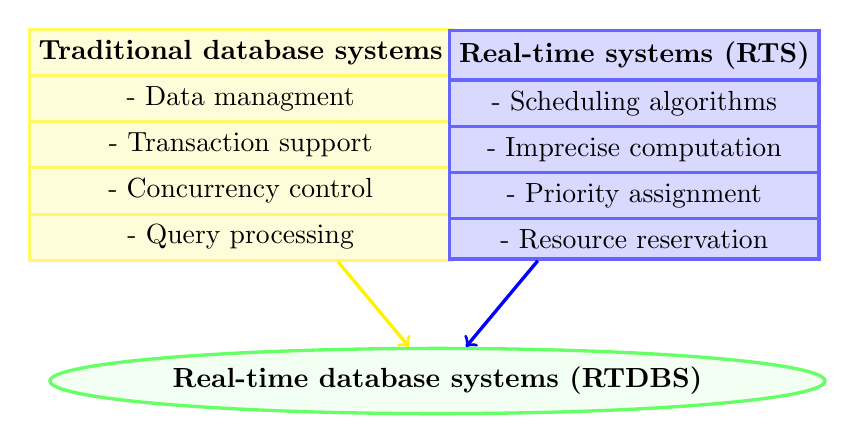
\begin{tikzpicture}[
roundnode/.style={ellipse, draw=green!60, fill=green!5, very thick, minimum size=5mm},
spitrecnode1/.style={rectangle split, rectangle split parts=5,draw, text centered, draw=yellow!60, fill=yellow!15, very thick, minimum size=2mm},
spitrecnode2/.style={rectangle split, rectangle split parts=5,draw, text centered, draw=blue!60, fill=blue!15, very thick, minimum size=2mm},
]

%Nodes
\node[spitrecnode1] at (0,3) (DBS) {\textbf{Traditional database systems} \nodepart{second} - Data managment \nodepart{third} - Transaction support \nodepart{fourth} - Concurrency control \nodepart{five} - Query processing};
\node[spitrecnode2] at (5,3) (RTS) {\textbf{Real-time systems (RTS)} \nodepart{second} - Scheduling algorithms \nodepart{third} - Imprecise computation \nodepart{fourth} - Priority assignment \nodepart{five} - Resource reservation};
\node[roundnode] at (2.5,0) (RTDBS) {\textbf{Real-time database systems (RTDBS)}};

%Lines
\draw [->] (DBS) [very thick, yellow] -- (RTDBS);
\draw [->] (RTS) [very thick, blue]-- (RTDBS);

\end{tikzpicture}
}
\\
\hline
\end{tabular}	
	\caption{Real-time database systems}
	\label{fig:RTDBS}
\end{figure} 

\indent To understand the need for real-time databases, it is important to have a high level overview of some of the various applications that employ real-time databases. While the applications can be endless, a big picture understanding of a few of them will provide context that can be expanded to almost any other application. Self-driving vehicles employ numerous sensors for geo-location (such as latitude/longitude and car velocity) and object detection (microwave radar and other such sensors) to make real-time decisions.  These decisions are the result of the derived data from various dynamic and static data inputs.  Flight control software, which a key example of this has been in the news lately with the Boeing Super Max flight control software, was designed to make adjustments to flight control surfaces based on sensor inputs.  Industrial control systems which can take various real-time inputs to make changes to industrial process (i.e. a simple pressure temperature relationship which can adjust energy input based on sensors for pressure and temperature). Lastly electrical grid operations employ various sensors to control grid operations based on energy demand or sensed faults to automatically re-route electrical distribution networks. This "smart grid" technology is used to prevent or minimize service disruptions or even cycle off customer's air conditioning units during times of high grid usage. These four examples all share the commonality that the state of the data at one point of time can be significantly different than it is in even a few milliseconds. Making determinations or predictions using stale data can be detrimental to the system and thus data correctness needs to be ensured before actions are taken as a result of the data.

\subsection{Transaction Properties}
Real-time transactions within a real-time database are characterized by distinct properties: the nature of real-time constraints, the arrival pattern, and the data-access type~\cite{Erickson}. Real-time constraints relate to the urgency of the transaction and the effect of missing its deadline. These constraints can be categorized into three types; hard, soft, and firm~\cite{Halpin}. Hard real-time constraints require that deadlines cannot be missed and the deadline is guaranteed by the system. An example of this would be velocity for a self driving vehicle. Every predefined interval would require that both speed and direction are obtained so that the exact location can be known within an area of uncertainty based upon the accuracy of the sensors employed. With this information the vehicle knows where it is and where it will be at the next predefined interval, and thus must be guaranteed to occur for the system to operate.
Soft real-time transactions are not guaranteed by the system and can only result in the performance degradation of the system if the deadline is missed. Again, looking at an example of a self-driving vehicle, a soft constraint could be a GPS location of the vehicle. While a continuous latitude and longitude helps to shrink the overall area of uncertainty of the cars location, at times that GPS may not be available such as when going through a tunnel. The area of uncertainty of the vehicle's location based upon the vehicle's velocity may grow and the parameters relied upon for this may degrade to account for this until the GPS location is regained and compared to the velocity calculated position of the vehicle. As a result of this degraded performance,  parameters such as stand-off distance to the car in front of you may increase.
Firm constraints are a special case of soft constraints in that when the deadline expires, the constraint is killed. Again employing an example of a self driving vehicle, this could be associated with a sensor that detects if the headlights should be on or not. If the sensor that detects outside illumination does not return a value to the database, the lights would remain on until a valid detection is received that would indicate that the lights could be turned off.\\
\indent A second property employed with real-time transactions is the arrival pattern of transactions. Arrival pattern transactions refer to the time interval transaction are execution. These arrival patterns can be periodic, aperiodic, or random~\cite{Erickson}.  Periodic transactions are transactions that are periodically executed within the real-time database. Aperiodic transactions means there is not a regular time interval between the executions of transactions~\cite{Erickson}. Again looking at an example of a self driving vehicle. The velocity sensors (speed and direction) would be periodic since they are required to be executed at a fixed interval to ensure the location of the car is known and can be predicted for the next interval. The GPS sensors would be aperiodic since the data is available when they are available, but if in a tunnel or blocked by a building they would not be able to be executed. Random would be the object detection sensors since objects would appear at random as the vehicle is moving. Random transactions would only execute when an object is detected.\\
\indent The third transaction property of real-time databases relate to the data access type and can be categorized as: write transactions, update transactions, and read transactions. As their names suggest, write transactions obtain the state of the environment and write to the database, update transactions derive new data and store them into the database, and read transactions read the data from the database and send them~\cite{Erickson}.\\
\indent As with traditional databases, real-time databases must guarantee internal consistency through ACID properties. A real-time database defines these properties as follows. Atomicity is applied for subtransactions, where subtransactions must be wholly executed or no transaction can be considered from them. Consistency requires that the transaction execution must always change the consistent state of the database in another consistent state. Isolation requires actions of a transaction be visible by other transactions before it commits. Durability requires the actions of a transaction need not be persistent, since both data and transactions have temporal validity~\cite{Halpin}.
\indent The implementation of a real-time database, vice a relational database, is required for various reasons. These reasons include applications in which the volume of data is large, the responses depend on multiple values, responses to aperiodic events are required, or when there are constrained timing requirements that must be met ~\cite{Halpin}.  The reason for this is that unlike relational database systems, real-time database systems must not only maintain database integrity but they must also meet the urgency of transaction executions.
\subsection{Data Properties}
The data correctness of a real-time database is more difficult to assure than for a relational database since the data is dynamic and the state of the database changes constantly.  The correctness of the real-time database implies that all usual consistency constraints are satisfied as well as being able to execute transactions within specified timing constraints and satisfy temporal consistency of the data. This temporal data consistency is concerned with the relative recency of data within the database. Data correctness for a real-time database is assured by both logical and temporal consistency~\cite{Kang}. Transactions are only considered correct if they finish within their deadlines using valid data~\cite{Buchmann}.\\
\indent The data within the database can be classified as static or dynamic. Static data correctness can be guaranteed by logical consistency since it has not become outdated. Dynamic data changes to reflect the real-world state which makes logical consistency impossible and thus temporal data consistency must be used~\cite{Kang}.\\
\indent Since dynamic data is time-stamped, validity intervals can be used to assure the consistency between the state represented by the database content and the actual state of the environment. The absolute validity interval ($avi$) is defined between the environment state and the value reflected in the database~\cite{Halpin}. This can be used to determine if the data is temporally inconsistent by comparing the data time-stamps. For instance, data $x$ is temporally inconsistent if $Current_{time} - Current_{timestamp}(x)>avi(x)$.\\
\indent The relative validity interval ($rvi$) is defined among the data used to derive other data~\cite{Erickson}.  For instance, in a real-time database that contains object speed $s$ and direction $d$, a moving object's position can be defined by the object's location at the previous time stamp plus the velocity vector times the elapsed time. $position_{t1} = position_{t0} + velocity_{average} (time_{t1} - time_{t0})$. As long as the time interval between the object's speed and direction is small (as a function of the object's ability to change speed and direction), the error of the average velocity will also be small. Therefore the recency of the $s$ vector is relative to the recency of the $d$ vector in such that the actual position of an object can be found with the $s$ and $d$ vectors for any given time. As discussed, this is relative to the objects ability to change speed and direction so the recency of data for a jet plane would have a much smaller relative validity interval required than say for a typical on-road vehicle.\\
\indent To best understand the data property requirements and how they are implemented for a real-time database, a simple example can be employed. Figure~\ref{fig:Example} depicts a simple real-time database with two sensors which are writing parameters to the database in real-time and one derived variable which updates to the real-time database based upon the sensors. $S_1$ and $S_2$ are dynamic sensors which can be represented by $x:(value, avi, timestamp)$. For this example we will again use our self driving vehicle example for context. $S_1$ will represent the direction component of the velocity vector based upon a compass heading; $0^o$ equates to North, $90^o$ equates to East, $180^o$ equates to South, and $270^o$ equates to West. $S_2$ represents the speed component of the velocity vector in miles per hour (mph). $D_1$ is a derived variable for the displacement using $S_1$ and $S_2$. In order for the the dynamic data to be temporally consistent, both the absolute and relative validity interval must be satisfied. For this example the design constraints for the vehicle are  $avi(S_1) = 5 ms$ and an $avi(S_2)=10 ms$. $D_1$ is derived from $S_1$ and $S_2$ and we assign a relative  validity interval $rvi(D_1)=2 ms$. This says that the direction component of the velocity vector must not be "older" than $5 ms$, the speed component cannot be "older" than $10 ms$, and that the relative difference time between the speed and direction components cannot be greater than $2 ms$.
\begin{figure}[h] % [h] forces the figure to be output where it is defined in the code (it suppresses floating)
\begin{tabular}{| p{0.45\textwidth}|}
\hline
\\
	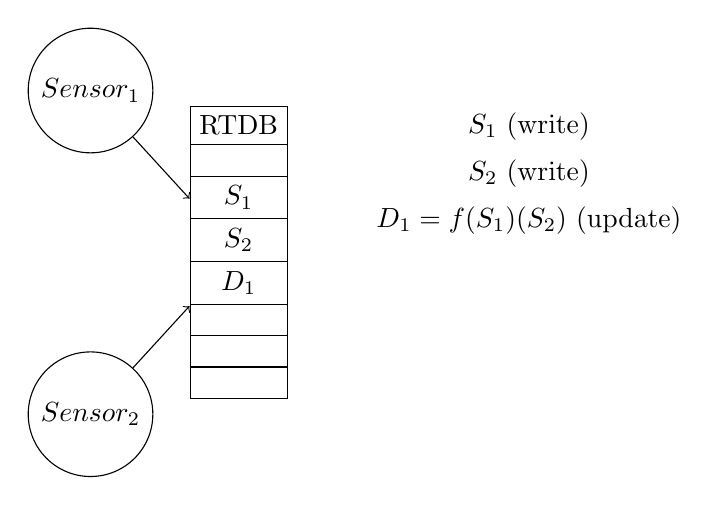
\begin{tikzpicture}[
roundnode/.style={circle, draw=black, thin, minimum size=5mm},
blankroundnode/.style={circle, draw=white, thin, minimum size=5mm},
spitrecnode/.style={rectangle split, rectangle split parts=8,draw, text centered, thin, minimum size=2mm},
spitrecnodeB/.style={rectangle split, rectangle split parts=8,draw=white, text centered, thin, minimum size=2mm},
]
%Nodes
\node[roundnode] (S1) {$Sensor_1$};
\node[blankroundnode] (SB1) [below=of S1] {};
\node[roundnode] (S2) [below=of SB1] {$Sensor_2$};
%\node[blankroundnode] (SB2) {};
%\node[blankroundnode] (SB3) {};
\node[spitrecnode] (RTDB) [right=of SB1] {RTDB \nodepart{third} $S_1$ \nodepart{fourth} $S_2$ \nodepart{five} $D_1$};
\node[spitrecnodeB] (DER) [right=of RTDB] {$S_1$ (write) \nodepart{second} $S_2$ (write) \nodepart{third} $D_1 = f (S_1) (S_2)$ (update)};
\path[every node/.style={font=\sffamily\small}]   
	(S1) edge [->] node [below] {} (RTDB)
		(S2) edge [->] node [below] {} (RTDB);
%	(A) edge [->] node [below] {$1$} (C)
   % (C) edge [->] node [below] {$1$} (B)
	%(B) edge [->, bend right=45] node [below] {$7$} (S);

\end{tikzpicture}

\\
\hline
\end{tabular}	
	\caption{Simple Real-time database system}
	\label{fig:Example}
\end{figure} 
\begin{table}[h] % [h] forces the figure to be output where it is defined in the code (it suppresses floating)
\begin{center}
\begin{tabular}{|c|c|c|c|c|c|}
\hline
Case & Time & $S_1$ & $S_2$ & temporal consistency\\
\hline
1& 25 & (124,5,20) & (16,10,22)& Assured\\
\hline
2& 25 & (124,5,20) & (16,10,24) & Not Assured\\
\hline
3&25&(124,5,19) & (16,10,17) & Not Assured\\
\hline
\end{tabular}
\end{center}
	\caption{Temporally consistency data}
	\label{tab:Example}
\end{table} 

\indent Looking at case 1 from Table~\ref{tab:Example} you can see that the $avi$ values for both $S_1$ and $S_2$ are met:
\begin{eqnarray}
avi(S_1) =(25-20=5)\leq 5 \\
avi(S_2)=(25-22=3) \leq 10
\end{eqnarray}
Looking at the $rvi(D_1)$ it can be seen that 
\begin{eqnarray}
rvi(D_1) = (22-20 = 2) \leq 2
\end{eqnarray}
 so relative temporal consistency is assured. In case 1 both the relative and absolute intervals are met so in case 1 temporal consistency is assured.
\\
\indent In case 2 on the other hand, the absolute intervals are met but 
\begin{eqnarray}
rvi(D_1) = (24-20 =4) > 2
\end{eqnarray} 
so the relative interval is not met and temporal consistency is not assured.\\
\indent In case 3 the $avi$ value for $S_2$ is met:
\begin{eqnarray}
avi(S_2) =(25-17=8)\leq 10
\end{eqnarray}
but the $avi$ value for $S_1$ is not met:
\begin{eqnarray}
avi(S_1) = (25-19=6)>5
\end{eqnarray}  
even when the $rvi$ for $D_1$ is met:
\begin{eqnarray}
dvi(D_1)=(19-17=2) \leq 2
\end{eqnarray}   so the temporal consistency is not assured. In both case 2 and 3, the transaction are not considered correct because the data would not be considered valid.

\section{Employing a real-time application with a real-time database}
\subsection{Google Firebase}
The Firebase Realtime Database is a cloud-hosted database in which data is stored as JSON and synchronized in real-time to every connected client. Firebase allows cross-platform apps to share one real-time database instance and automatically receive updates with the newest data. Data is persisted locally, and even while offline, real-time events continue to fire, giving the end user a responsive experience. When the device regains connection, the Realtime Database synchronizes the local data changes with the remote updates that occurred while the client was offline, merging any conflicts automatically\cite{Firebase}.
\indent The Firebase real-time database is a NoSQL database and has different optimizations and functionality as compared to a relational database.  Instead of typical HTTP requests, the Firebase real-time database uses data synchronization every time data changes, any connected device receives that update within milliseconds~\cite{Firebase}. Firebase apps remain responsive even when offline because the Firebase real-time database SDK persists data to disk. Once connectivity is reestablished, the client device receives any changes it missed, synchronizing it with the current server state\cite{Firebase}.
Firebase can be accessed directly from a mobile device or web browser meaning there’s no need for an application server. Security and data validation is available through the Firebase real-time database security rules which are expression-based rules that are executed when data is read or written~\cite{Firebase}.

\subsection{Cheap Gas Finder Application}
An application to update real-time gas prices as reported by users to all other users was developed and hosted on Google Firebase. The application enabled cross-platform functionality for both both web based and Android based functionality. The application allows a user to enter the price of gas on their application for a particular gas station and in real-time, update all other connected users of the price. The web based application can be seen in Figure~\ref{fig:WebApp} and the Android based application can be seen in Figure~\ref{fig:Android}. The active web application is hosted at the following url: \color{blue}\underline{\texttt{https://project-30a72.web.app}}.\color{black}

\begin{figure}[h] % [h] forces the figure to be output where it is defined in the code (it suppresses floating)
\begin{tabular}{| p{0.45\textwidth}|}
\hline
\begin{center}
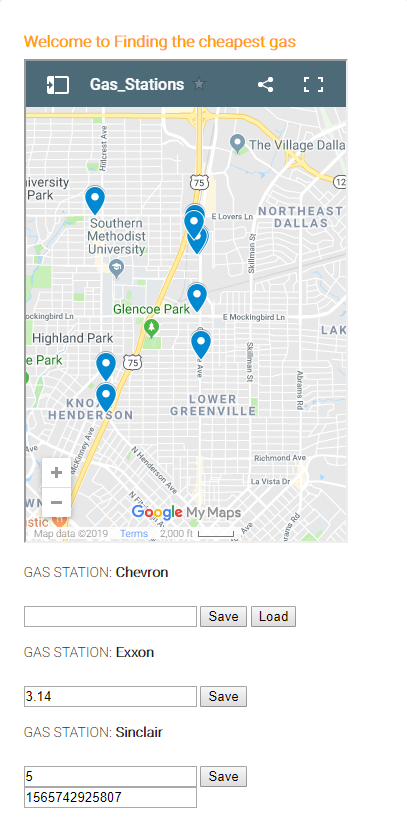
\includegraphics[scale=.35]{../graphics/WebApp.png}
\end{center}
\\
\hline
\end{tabular}	
	\caption{Web based Application for Cheap Gas Finder}
	\label{fig:WebApp}
\end{figure} 

\begin{figure}[h] % [h] forces the figure to be output where it is defined in the code (it suppresses floating)
\begin{tabular}{| p{0.45\textwidth}|}
\hline
\\
\begin{center}
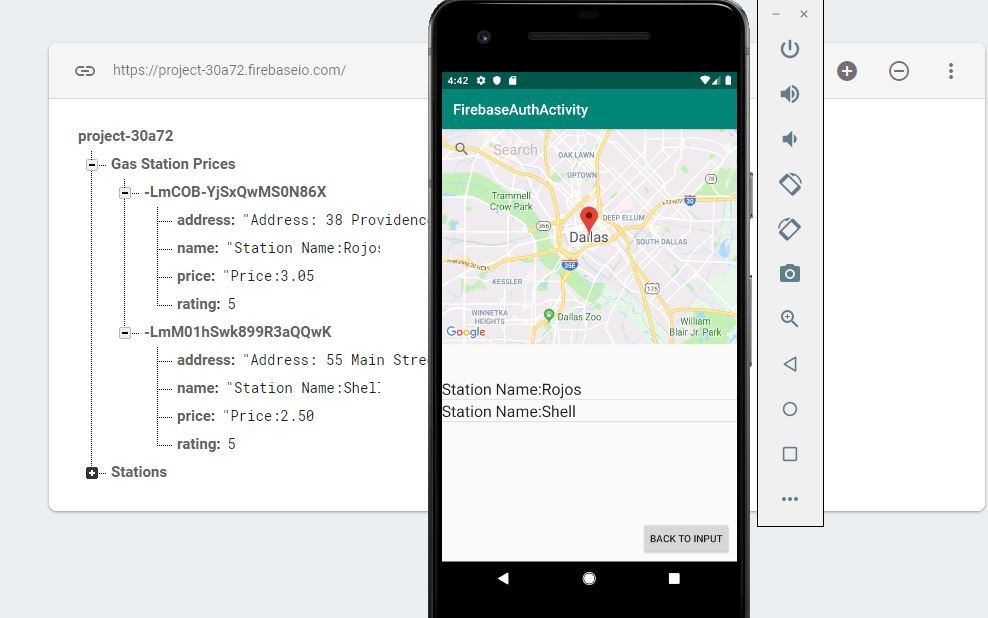
\includegraphics[scale=.35]{../graphics/SecondStationReadUpdatePicture3.JPG}\\
\end{center}
\\
\hline
\end{tabular}	
	\caption{Android Application for Cheap Gas Finder}
	\label{fig:Android}
\end{figure} 

The source code for both applications can be found in appendix~\ref{sec:SourceCode}. The web based application source code can be found in section~\ref{sec:SourceCodeWebApp} of the appendix and the Android based application source code can be found in section~\ref{sec:SourceCodeAndroidApp}.
\section{Connecting the Google Firebase RTDB}
One of the biggest challenges was connecting the Android application to the Firebase real-time database. This was accomplished in the following manner.
\subsubsection{packageID}
Each Android project comes with a “packageID” in the build.gradle file which is the file used to compile the application. Firebase needs this ID since it is what provides the connection from Firebase to the local application. This can be seen in Figure~\ref{fig:Step1}

\begin{figure}[h] % [h] forces the figure to be output where it is defined in the code (it suppresses floating)
\begin{tabular}{| p{0.45\textwidth}|}
\hline
\\
\begin{center}
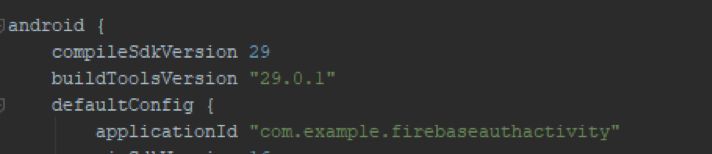
\includegraphics[scale=.6]{../graphics/Step1.png} \end{center}\\
\hline
\end{tabular}	
	\caption{Android Application packageID}
	\label{fig:Step1}
\end{figure} 

\subsubsection{Firebase Configuration File}
Firebase will then give generate a configuration file called \texttt{google-services.json}. This sets up the application with everything it will need when contacting the database to the application.  The \texttt{google-services.json} is then copied  into the application level folder.  This can be seen in Figure~\ref{fig:Step2}
\begin{figure}[h] % [h] forces the figure to be output where it is defined in the code (it suppresses floating)
\begin{tabular}{| p{0.45\textwidth}|}
\hline
\\
\begin{center} 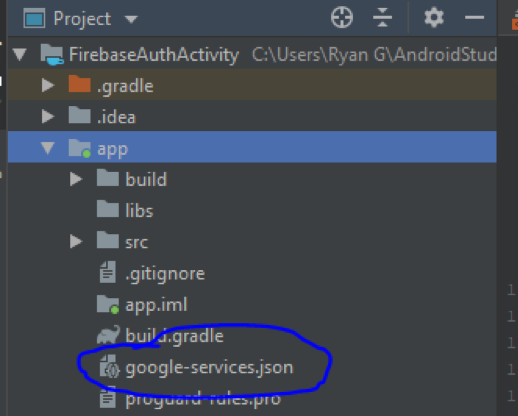
\includegraphics[scale=.6]{../graphics/Step2.png} \end{center}\\
\hline
\end{tabular}	
	\caption{Android Application packageID}
	\label{fig:Step2}
\end{figure} 

\subsubsection{Adding Implementations}
To get the application to read the json file when it needs to, go back to the build.gradle file and add the implementations into the dependencies setup to be able to utilize the commands the json configuration file has provided.  This can be seen in Figure~\ref{fig:Step3}
\begin{figure}[h] % [h] forces the figure to be output where it is defined in the code (it suppresses floating)
\begin{tabular}{| p{0.45\textwidth}|}
\hline
\\
\begin{center} 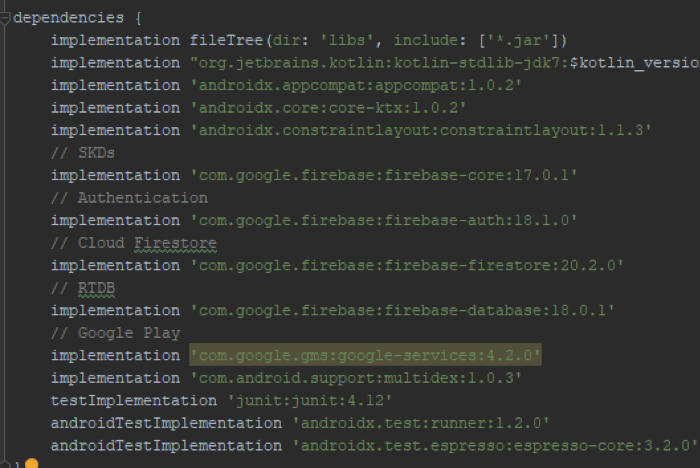
\includegraphics[scale=.6]{../graphics/Step3.png} \end{center}\\
\hline
\end{tabular}	
	\caption{Adding implementations to build.gradle}
	\label{fig:Step3}
\end{figure} 

\subsubsection{Application Building}
Now the application can be built making all variables and layout.  When variable need to be pushed to the database, these commands will write directly to the Firebase real-time database in a collection called \texttt{Gas Station Prices} at the push of a button.   This can be seen in Figure~\ref{fig:Step4}
\begin{figure}[h] % [h] forces the figure to be output where it is defined in the code (it suppresses floating)
\begin{tabular}{| p{0.45\textwidth}|}
\hline
\\
\begin{center} 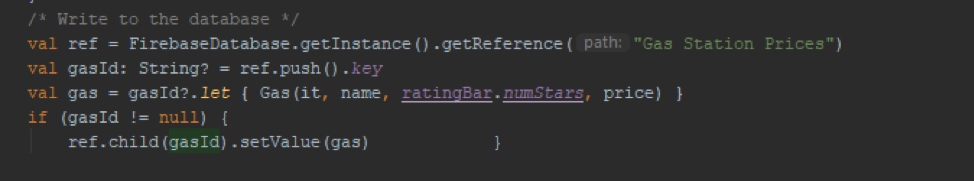
\includegraphics[scale=.5]{../graphics/Step4.png} \end{center}\\
\hline
\end{tabular}	
	\caption{Build Application}
	\label{fig:Step4}
\end{figure} 

\subsubsection{Application Verification}
The basic setup of the app in action can be seen in Figure~\ref{fig:Step5} and then verify what gets written to the database as seen in Figure~\ref{fig:Step6}. 
\begin{figure}[h] % [h] forces the figure to be output where it is defined in the code (it suppresses floating)
\begin{tabular}{| p{0.45\textwidth}|}
\hline
\\
\begin{center} 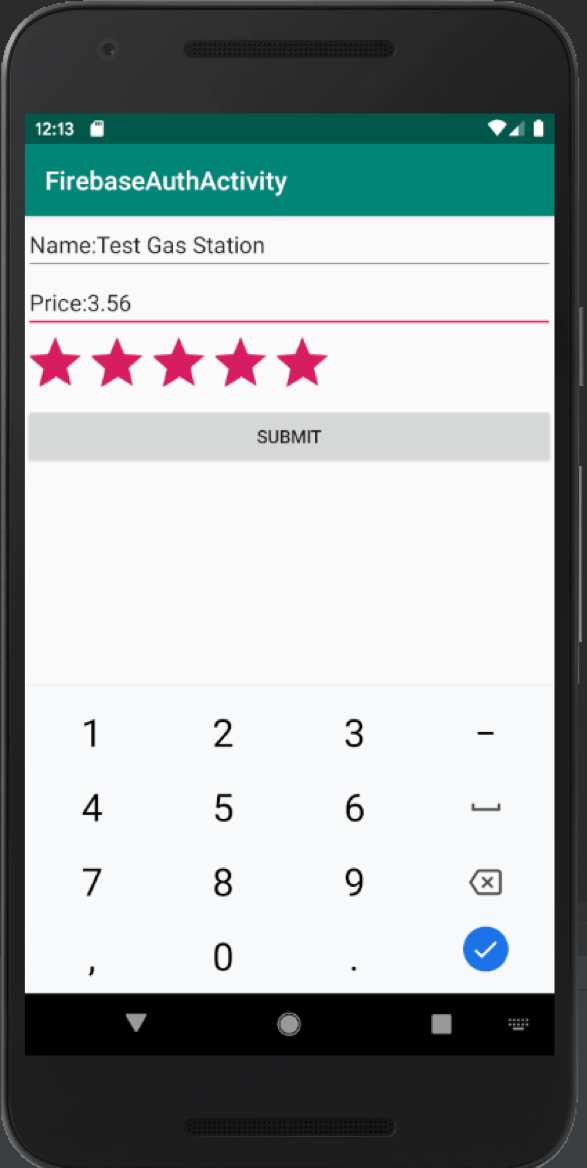
\includegraphics[scale=.35]{../graphics/Step5.png} \end{center}\\
\hline
\end{tabular}	
	\caption{Enter data into application}
	\label{fig:Step5}
\end{figure} 
\begin{figure}[h] % [h] forces the figure to be output where it is defined in the code (it suppresses floating)
\begin{tabular}{| p{0.45\textwidth}|}
\hline
\\
\begin{center} 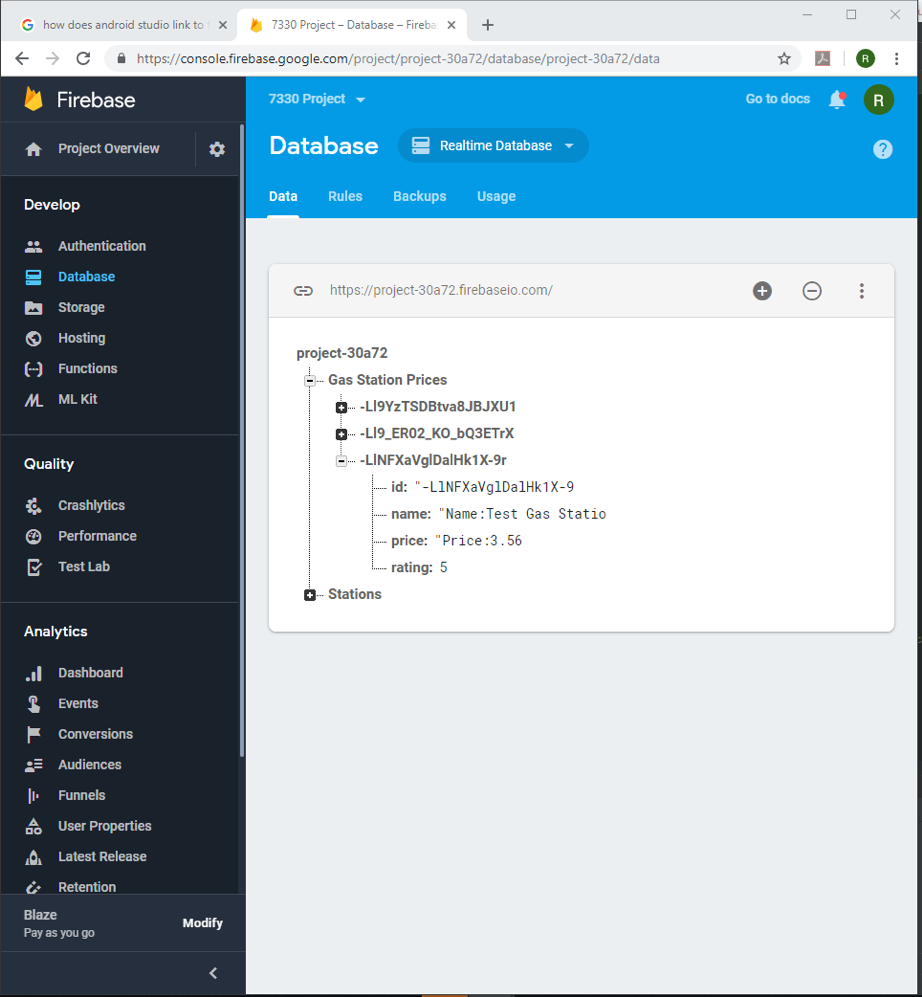
\includegraphics[scale=.4]{../graphics/Step6.png} \end{center}\\
\hline
\end{tabular}	
	\caption{Verify what is written to database}
	\label{fig:Step6}
\end{figure} 
\section{Conclusions}
Real-time databases provide the functionality of real-time processing for workloads that are constantly changing as needed for real-time systems. The traditional transaction and data properties of relational databases have to be extended to ensure not only logical consistency but temporal consistency in addition to the other usual consistency requirements. Without temporal data consistency, data within a real-time database can become stale. Since transactions are only considered correct if they finish within their deadlines using valid data, both transaction properties and data properties must be well understood for the system being employed.\\
\indent The Google Firebase real-time database provided the necessary tools to employ a cross-platform real-time application. The ability to perform real-time updates and broadcast them out to users was implemented and tested. While there was a steep learning curve in integrating the web based and Android based applications with Google Firebase, the end result was an application that provided real-time updates on gasoline prices that geo-located the stations on a Google map and transmitting those updates out to the various users using the Cheap Gas Prices applications.

%\bibliography{mybib}
%\bibliographystyle{ACM-Reference-Format}


\begin{thebibliography}{00}
\bibitem{Buchmann} Buchmann, A. Real Time Database Systems. Encyclopedia of Database Technologies and Applications. 2005
\bibitem{Lam} Lam, Kam-Yiu., and Kuo, Tei-Wei. Real-Time Database Systems Architecture and Techniques. Boston, MA: Springer US, 2002. 
\bibitem{Erickson} Erickson, John. Database Technologies: Concepts, Methodologies, Tools, and Applications. Hershey, PA: Information Science Reference, 2009. 
\bibitem{Halpin} Halpin, Terry. Selected Readings on Database Technologies and Applications. Hershey, PA: Information Science Reference, 2009. 
\bibitem{Kang} Kang, K. "qRTDB: QoS-sensitive real-time database. PhD thesis, Department of Computer Science, University of Virginia, Charlottesville. 2001
\bibitem{Han} Han, Song, Lam, Kam-yiu, Wang, Jiantao, Son, Sang H., and Mok, Aloysius K.  “Adaptive Co-Scheduling for Periodic Application and Update Transactions in Real-Time Database Systems.” The Journal of Systems \& Software 85.8 (2012): 1729–1743.
\bibitem{Firebase} “Firebase Realtime Database.” Firebase, Google, last retrieved July 13, 2019 from https://firebase.google.com/docs/database/


\bibitem{Jian} Jian-Feng, Lu, Chun-Yi, Wang, and Jie, Hu. “A High Performance Data Storage Method for Embedded Linux Real-Time Database in Power Systems.” Energy Procedia 16 (2012): 883–888.
\bibitem{Ferrucci} Ferrucci, Francesco, Bock, Stefan, and Gendreau, Michel. “A pro-active real-time control approach for dynamic vehicle routing problems dealing with the delivery of urgent goods.” European Journal of Operational Research 225 (2013): 130–141.


\bibitem{a8} Fernandes Ribeiro Neto, P.,  \& Yao, J. (2012). Exploration on the application of real-time database in ship electronic information system. Applied Mechanics and Materials, 263-266, 1414. 
\bibitem{a1} Han, Song et al. “Adaptive Co-Scheduling for Periodic Application and Update Transactions in Real-Time Database Systems.” The Journal of Systems \& Software 85.8 (2012): 1729–1743.
\bibitem{a2} Sun, Q et al. “Implementation of Massive Real-Time Database System Using Network Sensors and Sector Operation.” Sensors \& Transducers 174.7 (2014): 123–128.

\bibitem{a4} S. Samaiya and M. Agarwal, "Real time database management system," 2018 2nd International Conference on Inventive Systems and Control (ICISC), Coimbatore, 2018, pp. 903-908.

\bibitem{a6} RTDB: A Memory Resident Real-Time Object Database. United States. Dept. of Energy. Office of Energy Research, 2003
\bibitem{a7} Huang, K., Zhang, J., \& Yao, J. (2012). Exploration on the application of real-time database in ship electronic information system. Applied Mechanics and Materials, 263-266, 1414. 



\end{thebibliography}

\onecolumn
\appendix{} 
\section{Source Code}
\label{sec:SourceCode}

\subsection{Source Code for WebAppIndex.html}
\label{sec:SourceCodeWebApp}

\lstinputlisting[
	caption=Web Application Source Code (WebAppIndexHTML.txt)., % Caption above the listing
	label=lst:WebAppSC, % Label for referencing this listing
	language=html, % Use SAS functions/syntax highlighting
	frame=single, % Frame around the code listing
	showstringspaces=false, % Don't put marks in string spaces
	numbers=left, % Line numbers on left
	numberstyle=\tiny, % Line numbers styling
	]{../code/WebAppIndexHTML.txt}

\pagebreak

\subsection{Source Code for Android Application}
\label{sec:SourceCodeAndroidApp}

\lstinputlisting[
	caption= gradle file that allows the app to implement SDK’s such as Firebase and Google Services for Google Maps.  (buildGradle.txt)., % Caption above the listing
	label=lst:buildGraddle, % Label for referencing this listing
	language=html, % Use SAS functions/syntax highlighting
	frame=single, % Frame around the code listing
	showstringspaces=false, % Don't put marks in string spaces
	numbers=left, % Line numbers on left
	numberstyle=\tiny, % Line numbers styling
	]{../code/buildGradle.txt}

\pagebreak
\lstinputlisting[
	caption= Provides functionality to the first page of the application allowing user to write to the firebase database (MainActivity.txt) , % Caption above the listing
	label=lst:MainActivity, % Label for referencing this listing
	language=html, % Use SAS functions/syntax highlighting
	frame=single, % Frame around the code listing
	showstringspaces=false, % Don't put marks in string spaces
	numbers=left, % Line numbers on left
	numberstyle=\tiny, % Line numbers styling
	]{../code/MainActivity.txt}

\pagebreak
\lstinputlisting[
	caption= Second page of the application containing Google Map (ReadActivity.txt) , % Caption above the listing
	label=lst:ReadActivity, % Label for referencing this listing
	language=html, % Use SAS functions/syntax highlighting
	frame=single, % Frame around the code listing
	showstringspaces=false, % Don't put marks in string spaces
	numbers=left, % Line numbers on left
	numberstyle=\tiny, % Line numbers styling
	]{../code/ReadActivity.txt}

\pagebreak
\lstinputlisting[
	caption= Layout structure for placement of the editText and Button fields which are given functionality from the MainActivity code (ActivityMain.txt) , % Caption above the listing
	label=lst:ActivityMain, % Label for referencing this listing
	language=html, % Use SAS functions/syntax highlighting
	frame=single, % Frame around the code listing
	showstringspaces=false, % Don't put marks in string spaces
	numbers=left, % Line numbers on left
	numberstyle=\tiny, % Line numbers styling
	]{../code/ActivityMain.txt}

\pagebreak
\lstinputlisting[
	caption= Lays out where the google map will be and where the database reads will be displayed (ActivityRead.txt) , % Caption above the listing
	label=lst:ActivityRead, % Label for referencing this listing
	language=html, % Use SAS functions/syntax highlighting
	frame=single, % Frame around the code listing
	showstringspaces=false, % Don't put marks in string spaces
	numbers=left, % Line numbers on left
	numberstyle=\tiny, % Line numbers styling
	]{../code/ActivityRead.txt}

\pagebreak
\lstinputlisting[
	caption= Lays out where the google map will be and where the database reads will be displayed(readGasFunction.txt) , % Caption above the listing
	label=lst:readGasFunction, % Label for referencing this listing
	language=html, % Use SAS functions/syntax highlighting
	frame=single, % Frame around the code listing
	showstringspaces=false, % Don't put marks in string spaces
	numbers=left, % Line numbers on left
	numberstyle=\tiny, % Line numbers styling
	]{../code/readGasFunction.txt}

\pagebreak
\lstinputlisting[
	caption= Called by MainActivity to allow input of data (address\, name\, price) and mapped to Android Screen through ActivityMain.xml (gasFunction.txt) , % Caption above the listing
	label=lst:gasFunction, % Label for referencing this listing
	language=html, % Use SAS functions/syntax highlighting
	frame=single, % Frame around the code listing
	showstringspaces=false, % Don't put marks in string spaces
	numbers=left, % Line numbers on left
	numberstyle=\tiny, % Line numbers styling
	]{../code/gasFunction.txt}
	
\end{document}
“Firebase Realtime Database.” Firebase, Google, last retrieved July 13, 2019, URL.